\chapter{Online multi-agent plan recognition}
\label{ch:plan_recognition}
\textbf{Loren Champlin, Salena Ashton, Liang Zhang, Clayton Morrison}

\section{Introduction}

Plan recognition is the ability to understand and recognize logical structures and patterns within a sequence of observed behavior. Developing this capability for our AI agent would allow it to infer the latent plan structures, strategies, and goals (i.e., ``plan explanations") of not only individual human agents but a team of agents as well. Producing these plan explanations contributes to the logical belief structures that the AI agent must maintain as part of its theory of mind and theory of teams \citep{Tambe_1997,Baker_Tenenbaum_2014}. Furthermore, an AI agent could use these inferred plan explanations to predict the teams' subsequent actions and to help develop potential interventions for increasing team performance. Our AI agent must recognize the conjoined plan explanations of multiple agents given our team search and rescue setting and demonstrate this capability online (i.e., as the team carries out their mission). While a highly sparse topic, there are a few existing "state of the art" approaches for online Multi-Agent Plan Recognition (MAPR). 

The most recent online MAPR approach by \citet{Argenta_Doyle_2017} uses an automated planner to produce feasible plan explanations by simulating potential sets of parameters, conditions, and plan structures needed to generate the observed behavior. Approaches of this type are known as \textit{plan recognition as planning approaches} \citep{Ramirez_Geffner_2009,Van-Horenbeke_Peer_2021}. The use of an automated planner requires constructing a symbolic representation of the problem domain in which MAPR is to be deployed, known as knowledge engineering. Plan recognition as planning approaches are typically highly expressive and are capable of solving plan recognition problems that involve high levels of logical reasoning. However, this high expressivity usually comes at the cost of the high computational complexity required by the automated planner \citep{Van-Horenbeke_Peer_2021}. \citet{Argenta_Doyle_2017} attempt to overcome this challenge by making several strict simplifying assumptions about their problem domain. Although, these assumptions reduce the computational complexity at the cost of expressivity (i.e., it limits the type of problems their approach can solve). Another limitation is that \citet{Argenta_Doyle_2017} only consider ``flat" knowledge representations, rendering their approach incapable of inferring more than just the end-goals that the agents are trying to achieve. However, human behavior tends to exhibit hierarchical structures or patterns such that simple actions are combined to produce more complex actions. In terms of having a complete theory of mind and theory of teams, an AI agent needs to understand how actions relate to each other at different levels of granularity and complexity, not just how they relate to the agents' end-goals. 

Our proposed method for online MAPR is also a \textit{plan recognition as planning} approach. Rather than make assumptions that limit the problems our approach can solve, we try to overcome the challenges of computational complexity by developing a highly efficient automated planning algorithm specialized towards doing online MAPR. Our automated planning algorithm combines the well-known Simple Hierarchical Ordered Planner (SHOP2) proposed by \citet{Nau_2003} and the Monte Carlos Tree Search (MCTS) single-agent plan recognition algorithm proposed by \citet{Kantharaju_Ontanon_Geib_2019}. We also draw heavy inspiration from known parsing algorithms for Probabilistic Context-Free Grammars (PCFG) \citep{Collins_2011}. As suggested by its partial adaption of the SHOP2 algorithm, our approach assumes that the agents' actions relate through a set of hierarchical structures or what is known as a hierarchical task network (HTN) \citep{Nau_2003,Russell_Norvig_2021}. As such, our approach produces the most likely task hierarchy, which is an instance of a HTN under specific initial conditions. These task hierarchies represent how actions relate to each other at different levels of granularity of complexity by showing how high-level actions (also known as compound tasks) can be decomposed into low-level actions. 

\section{Approach}
In a HTN domain representation, compound tasks are high-level actions that are composed of lower-level actions. These lower-level actions may be compound task themselves that need to be further decomposed or non-decomposable actions, which are sometimes referred to as primitive tasks or just actions \citep{Russell_Norvig_2021}. Depending on how abstractly a compound task is defined, there may be multiple sets of lower-level actions that could be combined to create the same compound task. These different sets of actions are known as ``methods", since they are different ways of decomposing the compound task \citep{Russell_Norvig_2021}. Additionally, methods typically have preconditions, which are specific conditions that must be satisfied by the current state of the problem domain for that method to be used for task decomposition. If a methods preconditions are satisfied, then that method is said to be applicable \citep{Russell_Norvig_2021}. Figure \ref{pr_fig:1} further illustrates the concepts of compound tasks, actions, methods, and task decomposition. In the illustration, both methods could applicable or only one of them could be applicable given the current state of the problem domain. In the former case, an automated planner must choose one of the methods for decomposition, leading to two different possible plans. Further details on HTN planning processes can be found in the automated planning literature. (e.g., the SHOP2 paper by \citet{Nau_2003}). 

\begin{figure}[h]
    \centering
    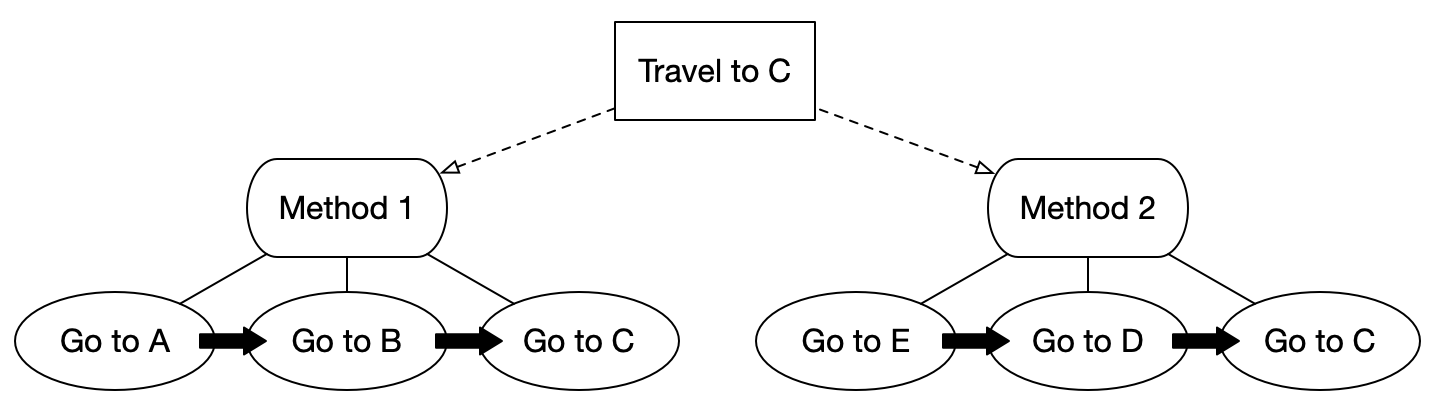
\includegraphics[width=1\textwidth]{images/htn_concepts}
    \caption{The compound task \textit{Travel to C} is shown to have two different methods for accomplishing the same task.} 
    \label{pr_fig:1}
\end{figure}

Our approach uses a HTN domain representation and an automated HTN planner to model the logical reasoning and decision-making process of a team of human agents. Compound tasks and methods are engineered in such a way as to represent the latent decisions that agents must make to complete their mission. From a generative perspective, these latent decisions are then what leads to the actions we observe from the human agents. With this concept in mind, we can have an automated planner generate a plan that matches the observed actions while recording the methods and task decompositions involved. As suggested in the introduction, this record is produced in the form of a task hierarchy which shows how compound task can be decomposed into the actions we observe. These task hierarchies are the plan explanations that give insight on the relationship between actions and the decision-making process of the agents. Figure \ref{pr_fig:2} illustrates the general concept of our online MAPR approach.

\begin{figure}[h]
    \centering
    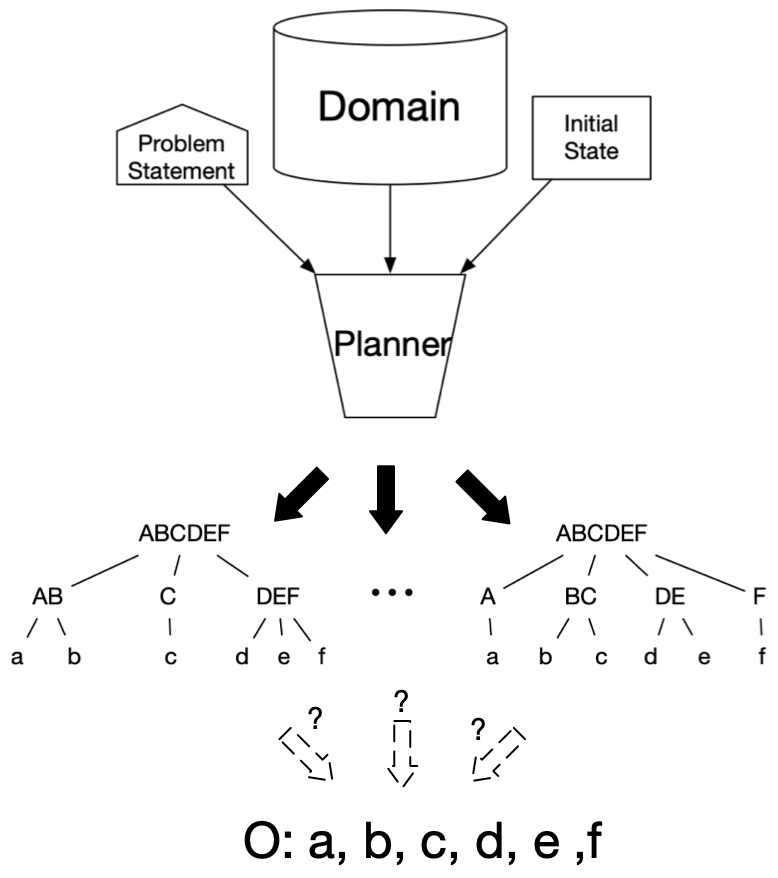
\includegraphics[width=1\textwidth]{images/pr_as_planning}
    \caption{In this illustration compound task are represented as groups of upper-case letters and actions are singular lower-case letters. Multiple potential task hierarchies can be generated for the same observed plan.} 
    \label{pr_fig:2}
\end{figure}

As seen in figure \ref{pr_fig:2}, it is possible that there are multiple plan explanations for same observed actions. However, rather than obtain all potential plan explanations given an observed sequence of actions, our approach should be yielding the most likely plan explanation. With this in mind, our approach assigns a conditional probability $p(m | \bigcap_{n \in M_t} c_n(s), s)$ for a method $m \in M_t$ for a compound task $t$. $c_n(s)$ denotes a function that is 1 if $n \in M_t$ is applicable to $t$ for the current state $s$, and 0 otherwise. The conditional probabilities are then defined as,

\begin{equation} \label{pr_eq:1}
p(m | \bigcap_{n \in M_t} c_n(s), s) = \begin{cases} \alpha  & c_m(s) = 1 \\ 0 & c_m(s) = 0 \\ \end{cases}
\end{equation}

\begin{equation}  \label{pr_eq:2}
\sum_{m \in M_t} p(m | \bigcap_{n \in M_t} c_n(s), s) = 1
\end{equation}

The value denoted by $\alpha$ in (\ref{pr_eq:1}) of each conditional probability must be predefined. As part of our approach we have formulated a training algorithm for learning these conditional probabilities, however that training algorithm is not detailed here. 

As suggested, an automated planner uses the methods defined in a HTN domain representation to decompose a compound task or set of compound tasks into a plan. This derivation of a plan is an analogous process to deriving a sentence from a PCFG. A PCFG contains a vocabulary of both non-terminal symbols and terminal symbols, as well as a set of derivation rules for replacing non-terminal symbols with a sequence of both non-terminal and terminal symbols \citep{Collins_2011}. Given an initial non-terminal symbol and applying rules successively eventually yields a sequence of only terminal symbols (i.e., a sentence) \citep{Collins_2011}. Similar to the methods of our HTN domain representation, each derivation rule is assigned a probability. Thus, given a specific derivation of a sentence (i.e., a specific set of derivations rules used), the probability of that derivation is the product of the probabilities of each rule used \citep{Collins_2011}. Given the similarities, we define the probability of a specific task hierarchy for a given plan in the same way. We denote $m_t$ as the applicable method chosen to decompose task $t \in \tau_\pi$, where $\tau_\pi$ is a set of tasks representing some task hierarchy used to generate a plan $\pi$. Using (\ref{pr_eq:1}), we have that,

\begin{equation} \label{pr_eq:3}
p(\tau_\pi) = \prod_{t \in \tau_\pi} p(m_t | \bigcap_{n \in M_t} c_n(s_t), s_t) 
\end{equation}

$s_t$ is current state prior to the decomposition of task $t$. Since our approach is for online MAPR, we want our plan explanations to consist of a partial task hierarchy that shows how the agents' latent decisions generates their plans up to the current time step. We denote the agents' observed partial plan (i.e., their observed sequence of actions up to some current time step) as $\pi^*$. We then simply replace $\pi$ in (\ref{pr_eq:3}) with $\pi^*$ to get,

\begin{equation} \label{pr_eq:4}
p(\tau_{\pi^*}) = \prod_{t \in \tau_{\pi^*}} p(m_t | \bigcap_{n \in M_t} c_n(s_t), s_t) 
\end{equation}

Using (\ref{pr_eq:4}), the objective of our approach is then to compute 

\begin{equation} \label{pr_eq:5}
\hat{\tau}_{\pi^*} = \argmax_{\tau_{\pi^*} \in T_{\pi^*}} p(\tau_{\pi^*})
\end{equation}

In (\ref{pr_eq:5}), $T_{\pi^*}$ denotes the set of all partial task hierarchies that match the observed partial plan $\pi^*$.

SHOP2 uses a depth first search (DFS) algorithm to generate plans and as such we could modify it to generate $T_{\pi^*}$ and then compute $\hat{\tau}_{\pi^*}$ by comparing $p(\tau_{\pi^*})$ for all $\tau_{\pi^*} \in T_{\pi^*}$ \citep{Nau_2003}. This is however an extremely computationally complex procedure and not a feasible method, especially for online MAPR where we would need to run this same computation many times. In general, using any automated planning algorithm to generate $T_{\pi^*}$ is not feasible. 

We argue that reasonable method would be to instead sample partial task hierarchies from $T_{\pi^*}$ and estimate $\hat{\tau}_{\pi^*}$ instead, this estimate being denoted $\bar{\tau}_{\pi^*}$. \citet{Kantharaju_Ontanon_Geib_2019} had come to this same conclusion in their development of an approach to do single-agent plan recognition using a domain representation based on Combinatory Categorical Grammars (CCGs). As mentioned in the introduction, they use a MCTS algorithm to sample the space of plans and find a reasonable estimate of the most likely plan explanation for an observed plan, reducing the computational complexity of their approach significantly. Using a similar concept, we modified the SHOP2 algorithm to use a MCTS algorithm as opposed to DFS. Although we will not go into full details here, MCTS samples solutions from the search space, which in our case are partial plan hierarchies matching the agents' observed partial plans. The search algorithm uses each sample to compute statistics about the search space that inform it where ``good" areas of the search space are according to some utility function \citep{Browne_Powley_Whitehouse_Lucas_Cowling_Rohlfshagen_Tavener_Perez_Samothrakis_Colton_2012,Kantharaju_Ontanon_Geib_2019}.In our case, our utility function is $p(\tau_{\pi^*})$, which the algorithm attempts to maximize. MCTS balances its search between completely unexplored areas and areas of the search space that have yielded good results before \citep{Browne_Powley_Whitehouse_Lucas_Cowling_Rohlfshagen_Tavener_Perez_Samothrakis_Colton_2012,Kantharaju_Ontanon_Geib_2019}. Given enough search time, our MCTS algorithm will eventually compute $\hat{\tau}_{\pi^*}$, although the needed search time would be roughly equivalent to what SHOP2 would need to do the same task. Therefore we must limit the search time allowed and have our algorithm return the best $\tau_{\pi^*}$ it can find under a predefined search time, which is our estimate $\bar{\tau}_{\pi^*}$. There is a high chance that $\bar{\tau}_{\pi^*}$ may only be a local optima, but it is likely to be a sufficiently probable plan explanation given a reasonable amount of search time. 

In terms of the Study 3 data, our approach heavily utilizes the json mission event messages coming from the message bus during the Search and Rescue mission trials. These messages are primarily used as the observations for our plan recognition algorithm, but are also used along with the video of the trials as source material for knowledge engineering our HTN domain representation. We also use the messages in our training algorithm to learn the conditional probabilities as defined in \ref{pr_eq:1} and \ref{pr_eq:2}. The specific input variables that we use in our approach from the message bus are as followed, 

\begin{itemize}
\item MinecraftEntity\_Event\_Triage\_Simulator
\item MinecraftEntity\_Event\_Roleselected\_Simulator
\item MinecraftEntity\_Event\_Proximityvictiminteraction\_Simulator
\item MinecraftEntity\_Event\_Playerfrozenstatechange\_Simulator
\item MinecraftEntity\_Event\_Tooldepleted\_Simulator
\item MinecraftEntity\_Event\_Markerplaced\_Simulator
\item MinecraftEntity\_Event\_Markerremoved\_Simulator
\item MinecraftEntity\_Event\_Markerdestroyed\_Simulator
\item MinecraftEntity\_Event\_Victimpickedup\_Simulator
\item MinecraftEntity\_Event\_Victimplaced\_Simulator
\item MinecraftEntity\_Event\_Rubbleplaced\_Simulator
\item MinecraftEntity\_Event\_Rubbledestroyed\_Simulator
\item MinecraftEntity\_Event\_Victimnolongersafe\_Simulator
\item MinecraftEntity\_Event\_Missionstate\_Simulator
\item MinecraftEntity\_Event\_Location\_Locationmonitor
\item MinecraftEntity\_Event\_Victimsexpired\_Simulator
\item MinecraftEntity\_Observation\_State\_Simulator
\item MinecraftEntity\_Observation\_Fov\_Fovtool
\item MinecraftEntity\_Event\_Dialogue\_Event\_Dialogagent
\end{itemize}

\section{Evaluation}
Since it would be extremely difficult to objectively confirm a teams latent decision process used for a mission trial, we have devised an alternative evaluation method for testing the performance of our online MAPR approach. The algorithm described in our approach section, can be reconfigured to project forward in time past the agents' observed partial plan, effectively allowing it to predict their most probable next actions using $\bar{\tau}_{\pi^*}$ as a reference point for the agents' latent decision-making process. We reason that the closer $\bar{\tau}_{\pi^*}$ is to the true value, the more accurate the action prediction will be. Using this concept, we can indirectly measure how well our approach works by measuring how accurate the action predictions are given $\bar{\tau}_{\pi^*}$.

While our algorithm could technically project forward to the end of a team's mission trial, we expect the prediction accuracy to increasingly diminish as the gap between the end of the projected plan and the observed partial plan increases. Instead we evaluate our algorithms performance by having it use $\bar{\tau}_{\pi^*}$ to predict only the next few actions. Given an observed plan from a completed mission trial, we can simulate having a teams' observed partial plan at a set time points in their mission. At these set time points, we can run our online MAPR algorithm and then have our planner predict the next few actions, and compare these predicted actions against the teams' true actions. 

We will compute two different types of accuracy measures, the action allocation accuracy and the action sequence accuracy, which are accuracy measures used in other MAPR literature \citep{Kim_Chacha_Shah_2015}. The action allocation accuracy is the ratio of how many predicted actions were correct out of the number of actions predicted \citep{Kim_Chacha_Shah_2015}. The action sequence accuracy is computed by first dividing the correctly predicted actions into pairs and then counting how many pairs are in the correct order (regardless of what actions they are predicted to have between them). This count is divided by what the count would be if all pairs were correctly ordered \citep{Kim_Chacha_Shah_2015}. The average action allocation and average action sequence accuracy over all trials will be computed for each prediction point, as well as average accuracy measures over all prediction points over all trials. 

We will also measure the rate at which our prediction accuracies decrease as we increase the number of actions predicted. This can be done by picking a singular prediction point for each trial and measuring the action allocation accuracy and action sequence accuracy as we increase the number of actions predicted. Increases in te number of actions predicted will be done at set intervals (e.g., 2 actions, 4 actions, 6 actions, etc).  Average accuracies will then be computed for each interval over all trials. 
